\chapter{Testrig}
%In this chapter I will describe the test rig, the test method, why it was chosen, what its limits are, how it works behind the scenes (mechanically/dynamically) how the tests are set up and so on.

%\begin{comment}  


\begin{figure}
\centering
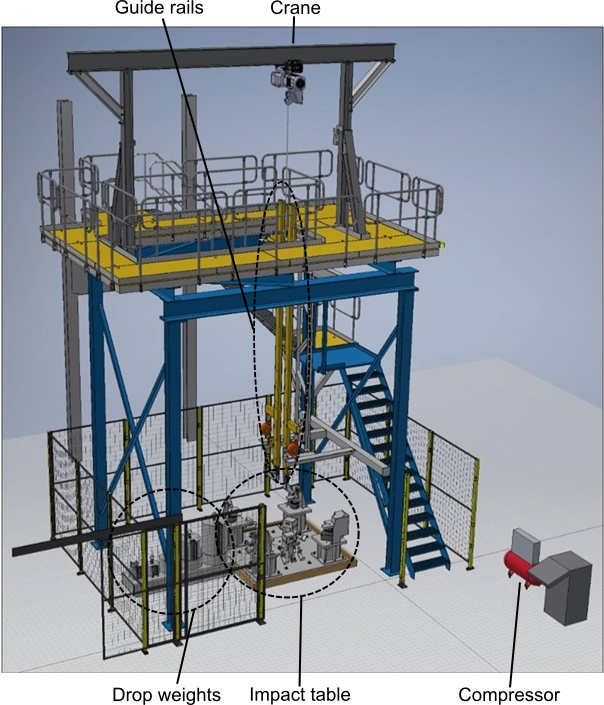
\includegraphics[width=\linewidth]{./pics/rig.png}
\caption{Drop test facility used at Kiirunavaara Mine}
\label{fig:drop}
\end{figure}

If you build a race track from scratch then drive a few laps on it and check the times, you have no idea if the car you're using is fast or slow. You need more data. As soon as you have driven a second car around the track you know which of the two is faster. The more cars you drive around the track the better your understanding of the capabilities of different cars ant the track itself becomes. 
It is the same for rock support systems and drop test rigs.

There is a lot of data available in literature, giving a general guideline of what to expect when running tests on various materials. But the test rig constructed at Kiirunavaara Mine is unique. Of course the results should be comparable to the results of other test rigs but they will be ever so slightly different.

To gain a baseline of the capabilities of the current support system and develop the test rig to its full potential is the aim of this thesis. With this baseline it is possible to compare future developments and ideas to the status quo and decide whether they are worth exploring further.  

The current test rig is depicted in \autoref{fig:drop}. As these were the first serious tests run with the rig, the setup and sensor array underwent some changes. Further enhancements are always possible, some are already planned, more will be discussed in the course of this thesis and the current setup is just a stepping stone on the way to a fully fledged testing facility. 

It is designed to test panels with dimensions of either as a circular plate with 0,8 m diameter or a square plate with 1,5 x 1,5 m. The impact energy can vary from 0 to almost 40 kJ. It is gravity based, which means the impact weight is in free fall. There's no direct measurement of the impact velocity. As the drop height is relatively low, < 4 m, air resistance negligible. The drop weight is supported by guide rails in order to hit the specimen in the center, the drop weights are fitted with low friction material. Currently there is no direct way to measure impact velocity, it is instead calculated, as per industry standard \autocite[13]{Crompton18}. %The impact energy is also only calculated. %TO DO fix energy calculation

\section{Energy Level}

The first challenge when testing the round samples was determining the energy level at which the specimen would crack but not break. The round concrete samples had a large variation in properties which made estimating the survivable impact energy even more interesting. %It did not seem sensible to calculate the energy needed through computer assisted means nor to spend hours trying to solve it analytically. 
This was done through trial and error. A question that posed itself during this process was turning the qualitative analysis of the destruction of the test samples, through visual inspection, into comparable numbers. 
\Textcite{canada96} divides broken samples into 4 categories. This categorisation was based on visual inspection of the post - test samples.

\begin{itemize}
    \item mild damage
    \item moderate damage
    \item severe damage
    \item destroyed
\end{itemize}

%Adopting this system seemed sensible, but as the tested specimen were all very homogeneous it was possible to implement a more quantitative system, based on the amount and width of cracks. 

\begin{figure}
    \centering
    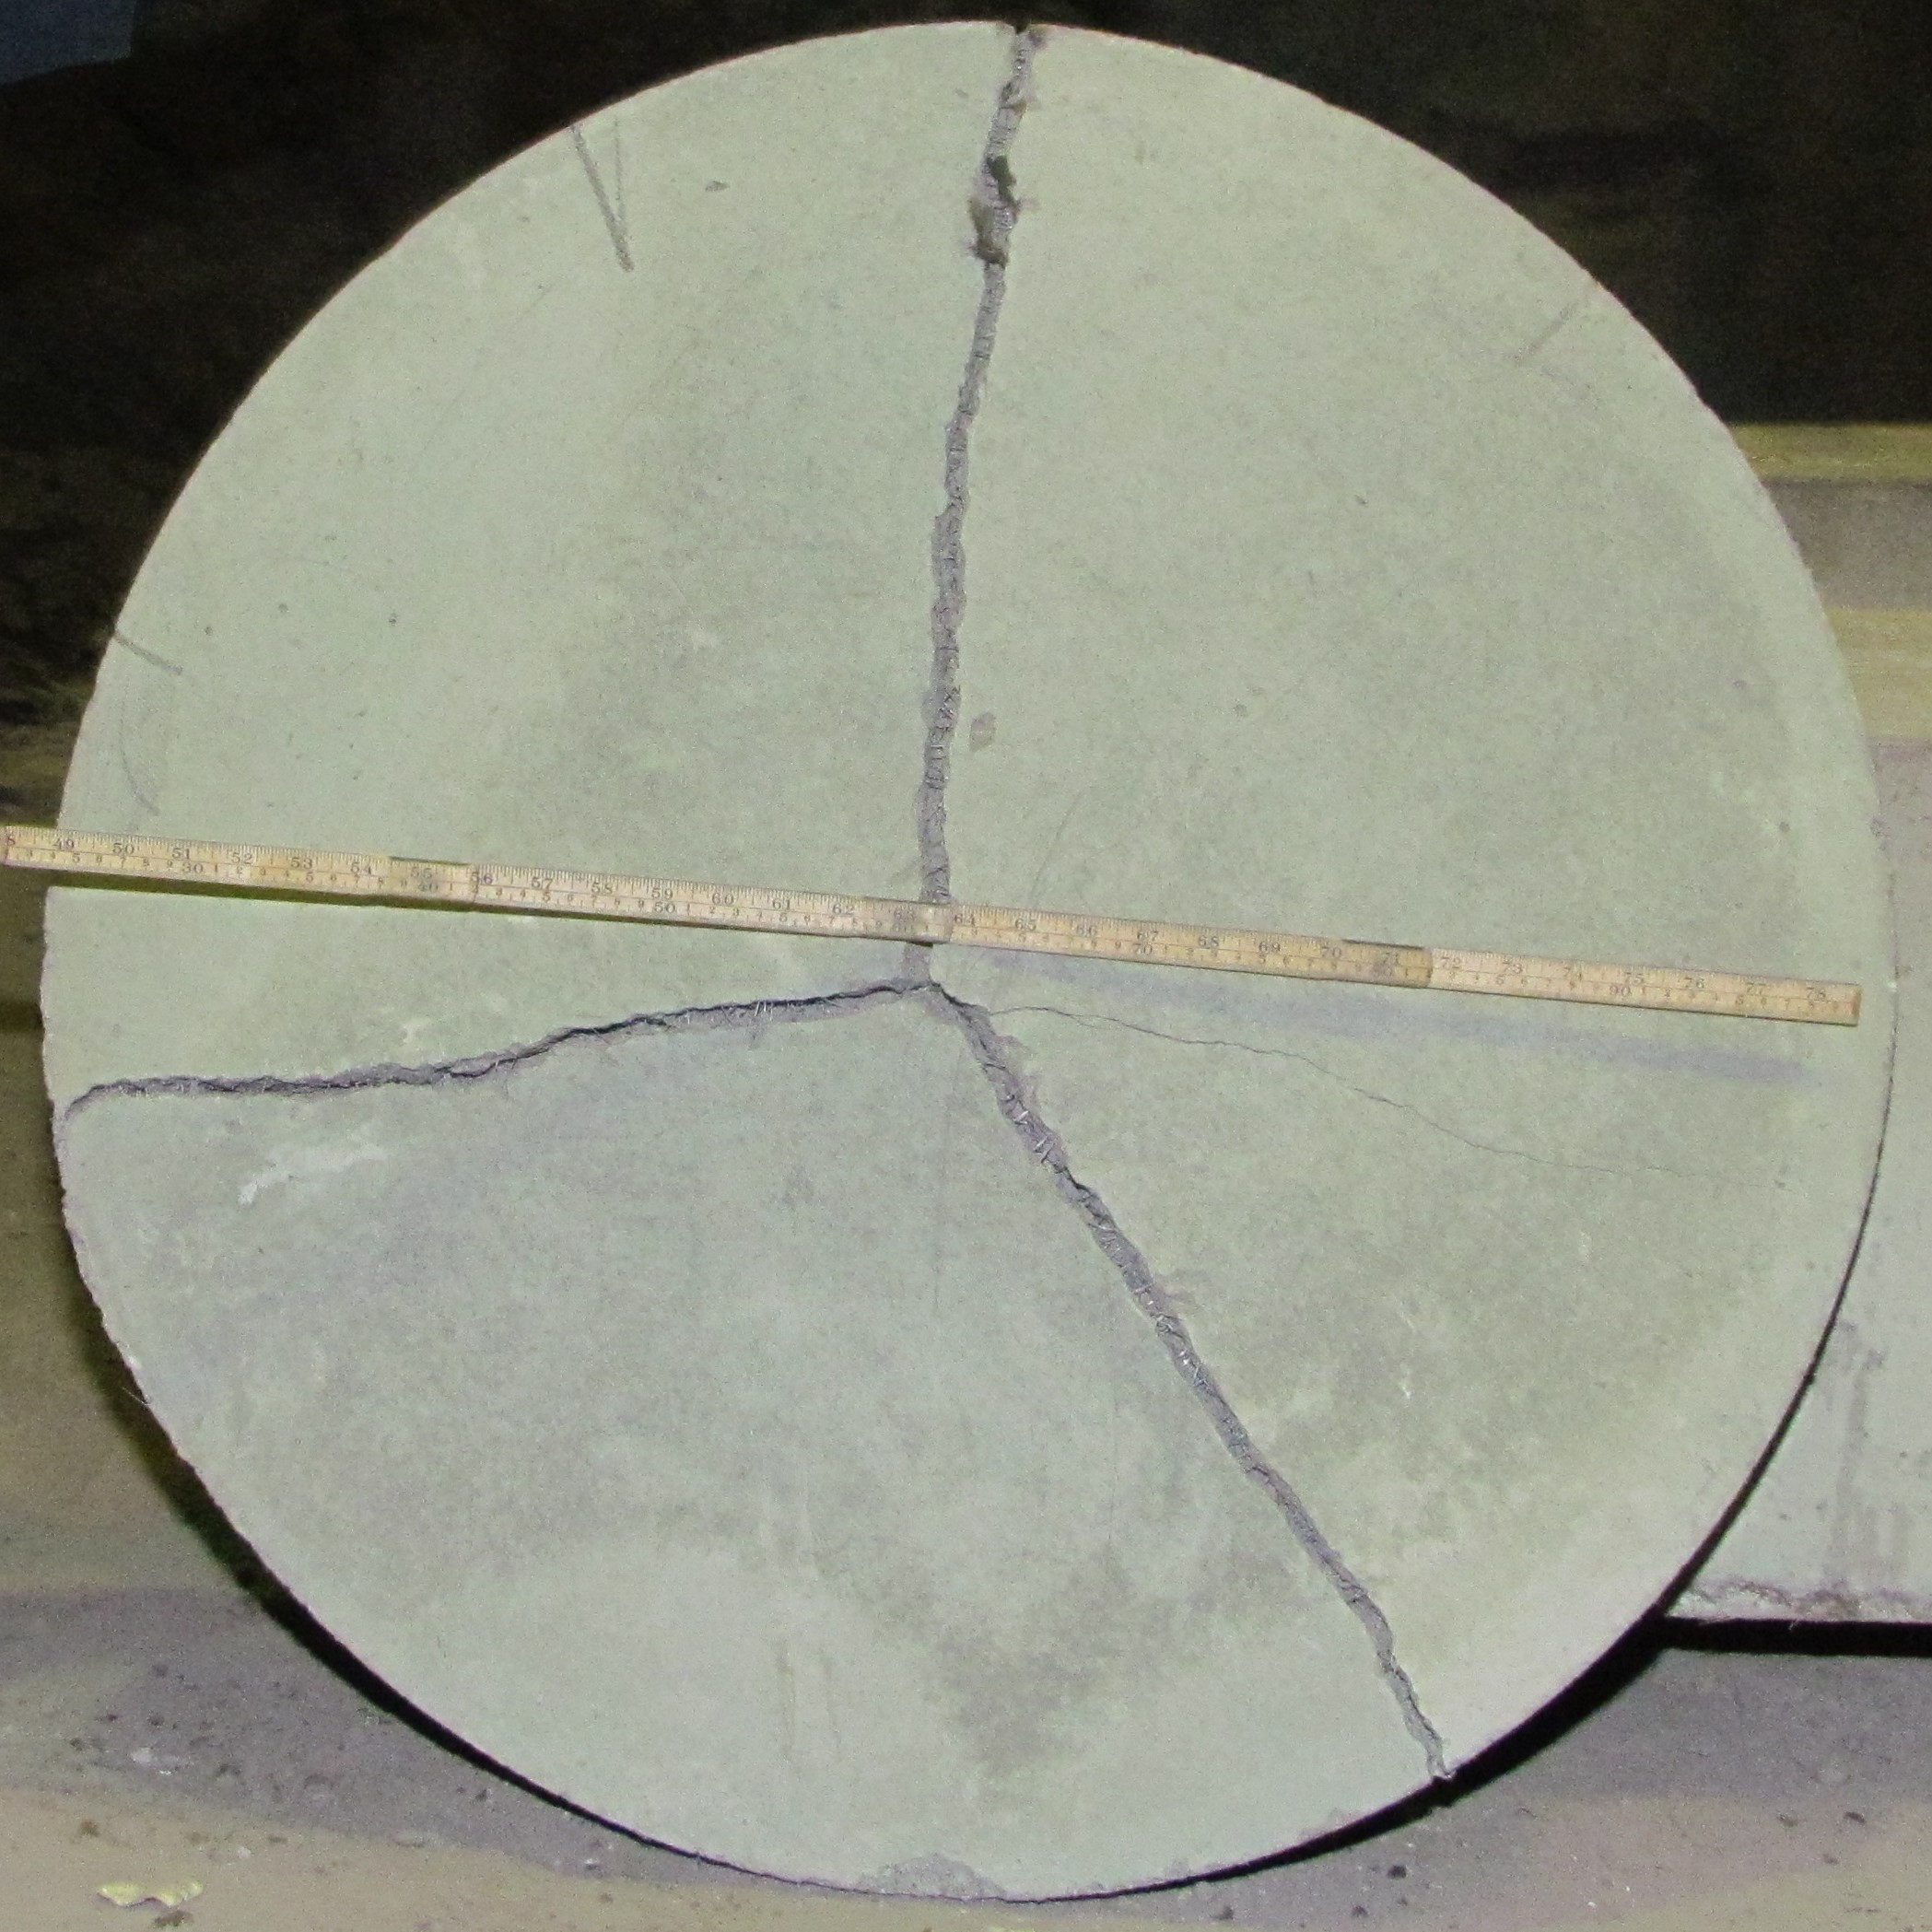
\includegraphics[width = 0.45 \linewidth]{appendix/2018-12-04_Rfrs_50_0,3.JPG}
    \caption{Crack pattern}
    \label{fig:crack_pattern}
\end{figure}

This system is qualitative and the measured results are influenced by the observer. A cautious operator might rate a sample as severely damaged, while a more confident observer could rate it as moderately damaged, for example. Therefore a more quantitative system was implemented.
As most of the energy is absorbed by forming cracks, the width of each crack was measured in 2 to 3 places and averaged. The length of the cracks was also recorded. From the crack length and width the surface of each crack could be calculated and therefore the entire crack surface of each specimen. For the round samples the most common failure mode was 3 large cracks (> 10 mm) accompanied by one or two small cracks (< 1 mm). See \autoref{fig:crack_pattern} or Appendix.

The median crack width was used to calculated the crack opening angle, to minimize distortion through outliers. The crack opening angle \(\Theta\) is defined as displayed in \autoref{fig:crack}. \(\Theta\) was calculated using \autoref{eq:theta}.

\begin{equation}\label{eq:theta}
    \Theta = 2 * \arctan{ \frac{width ~of~the~crack}{2 * thickness~of~the~panel}}
\end{equation}

\begin{figure}
\centering
\begin{tikzpicture}
%Crack angle stuff

\draw (6,0) coordinate (right);
\draw (4,0) coordinate (left);
\draw (5,5) coordinate (root);
\draw [thick] (0,5) -- (10,5)
(0,0) -- (left)
(right) -- (10,0);
% jagged cracks
\draw[thick]
(right)
-- ++(0.1,0.5)  
-- ++ (-0.1,0.2)
-- ++ (0.2, 0.1)
-- ++ (-0.2,0.1)
-- ++ (-0.1,0.8)
-- ++ (0.1, 0.2)
-- ++ (0.2, 0.2)
-- ++(-0.3, 0.3)
-- ++ (-0.1 , 0.4)
-- ++ (0.0, 0.3)
-- ++ (-0.3 , 0.4)
-- ++ (-0.2,0.4)
-- ++ (-0.2, 0.3) % end point
-- ++ (-0.3, -0.5)
-- ++ (-0.4, -0.2)
-- ++ (-0.2, -0.4)
-- ++ (0.1, -0.3)
-- ++ (0.1, -0.1)
-- ++ (-0.2, -0.4)
-- ++ (-0.4, -0.3)
-- ++ (0.1, -0.5)
-- ++ (-0.1,-0.2)
-- ++ (-0.3,-0.1)
-- ++ (0.2,-0.2)
-- ++ (0.1,-0.5)
-- (left)
;
\draw [gray]%[thick, dashed, red] %virtual crack 
(left) -- (root.south) 
coordinate[near start] (lmid)
-- (right) 
 ;
\draw [{Latex[length=3mm, width=1mm]}-{Latex[length=3mm, width=1mm]}] (4,-1) -- (6, -1)
node[midway, above]{width of crack};

%\draw [{Latex[length=3mm, width=1mm]}-{Latex[length=3mm, width=1mm]}] (lmid) arc [radius = 3.85, start angle = -101.31, delta angle = 22.62]
%node [midway, below] {\(\Theta\)} ;

% Draw the arc which center is (2,1)
\draw [{Latex[length=3mm, width=1mm]}-{Latex[length=3mm, width=1mm]}] ([shift=(-101.31:4cm)]root) arc [radius = 4cm, start angle = -101.31, delta angle = 22.62] node [midway, below] {\(\Theta\)} ;

\draw [{Latex[length=3mm, width=1mm]}-{Latex[length=3mm, width=1mm]}] (8,0) -- (8,5) 
node [midway, sloped, above] {thickness of the panel};


\end{tikzpicture}
\caption{Crack opening angle}
\label{fig:crack}
\end{figure}

%The energy absorbed by support elements was defined as the area underneath the force/displacement curve. 

\section{Failure Criteria}
Another problem was defining the failure criteria. \textcite{canada96} stated that rock support must be able to withstand quasi static loading conditions after a dynamic event.  %The construction of a quasi-static test rig is planned. The intend is 
For this a quasi-static test conducted with the same sample after a dynamic test would be interesting. This would make it possible to test the residual static capabilities of specimen that cracked during the initial dynamic test but did not break. With the current test rig it is not possible to perform such quasi static tests. 
%It was assumed, that as long as the tested specimen was only cracked but not broken after the dynamic test, it would still be able to withstand the static load.   

%For more ductile material such as chain-link mesh or welded mesh, which is scheduled to be tested in one of the successive campaigns, a maximum rate of displacement will have to be defined. This is due to the fact that some ductile materials are able deform beyond usability in an economic mining context. It simply does not make sense to lose large volumes of excavation space to deformations. 

%\textit{In - situ} deformations of the surface support mean that the excavation space, for example the cross section of a drift, is reduced. 
\textcite[344]{stacey01} stated: "as long as the excavation remains open and allows efficient operation, it has not failed." %. Excavations should be close to their stability limit. If no excavations fail, then it is probable that they are being too conservatively, and hence uneconomically, designed" 
With this quote in mind it obvious that allowing some degree of deformation is necessary when designing a support system. The question is how much local deformations an excavation survive without needing to be renovated.
%If this reduction is large enough, the drift becomes unusable. For example because vehicles, like dumper trucks, can no longer traverse the affected section. A costly renovation would become necessary to reestablish the usability of the drift. To avoid such situations a maximum deformation of the surface support must be defined as a failure criteria. 

%Only fibre reinforced concrete samples were tested up until now. Fibre reinforced concrete is stiff and will can not withstand large deformations before breaking. Which means that defining a failure criteria based on deformation was unnecessary. In successive testing campaigns, steel mesh will be tested. Welded mesh and chain-link mesh to be precise. Especially chain-link mesh has great displacement capacity. \autocite[575]{sme11}. 
Currently the test rig only has space for deformation of approximately 40 cm when testing square samples and even less for round samples.
For a round excavation with a diameter of 7 m a local deformation of 4 cm would mean a 6 \% loss in diameter. The usability of an excavation will most likely not be affected by deformations of this magnitude. 
%When considering  a round excavation with a diameter of 7 m . A lo
%Considering the current drift diameter is about 7 m a local deformation of 40 cm would mean approximately 5 \% loss of diameter. The usability of a drift will most likely not be affected by deformations of this magnitude. 
Therefore 40 cm are acceptable as failure criteria. There are plans to lift the impact table, to allow for deformations of up to one meter or more. Defining a maximum allowable deformation might have to be re-evaluated then.
The total deformation is the sum of the deformation of the tendon deformation and the surface support deformation. With the current test rig only the surface support deformation can be measured.
The amount of acceptable deformation depends on the size of the drift. A smaller drift can take less deformation before it becomes un-usable.

\section{Comparing Measured and Calculated Speed}
\label{sec:speed}

For one of the tests conducted on 2018-12-10 the theoretical and real impact velocity was calculated using the accelerometer measurements. The drop height was 1500 mm, the time from release of the weight to impact was taken from the accelerometer measurements. See \autoref{fig:speedcalc}. The weight started dropping at 346,963 seconds and the impact happened at 347,513 seconds. Therefore the weight dropped for \( t = 0,55~s \). The following calculations assume that \( g = 9,8~m/s \). 

The calculated peak velocity was calculated using \autoref{equ:vcalc}. The result was \( \hat{v}_{calc} = 5,42~m/s \).

\begin{figure}
    \centering
    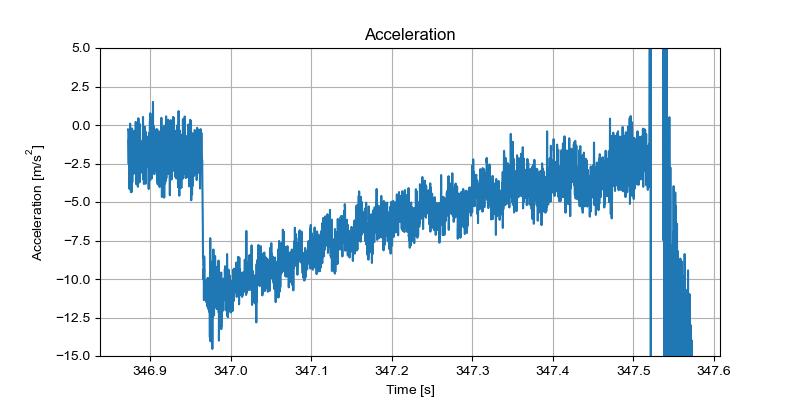
\includegraphics[width=0.9\linewidth]{pics/speedcalc.png}
    \caption{Acceleration during free fall used to calculate real drop speed}
    \label{fig:speedcalc}
\end{figure}

\begin{equation}
    \hat{v}_{calc} = \sqrt{2 * g * h}
    \label{equ:vcalc}
\end{equation}

The equations is derived by comparing the definitions of potential and kinetic energy as displayed in \autoref{equ:vcalcDer}. 

\begin{subequations}
    \begin{align}
    E_{pot} &= m * g * h \label{equ:Epot}\\
    E_{kin} &=  \frac{m * \hat{v}_{calc}^2 }{2} \\
    m * g * h &= \frac{m * \hat{v}_{calc}^2 }{2} \\
    \hat{v}_{calc} &= \sqrt{2 * g * h}
    \end{align}
    \label{equ:vcalcDer}
\end{subequations}


The indirectly measured peak velocity was calculated using \autoref{equ:vmes}.  The result was \( \hat{v}_{me} = 5,39 m/s \).

\begin{equation}
 \hat{v}_{mes} = g * t
 \label{equ:vmes}
\end{equation}

The equation is derived by considering the definition of speed as displayed in \autoref{equ:vmesDer}.
\begin{subequations}
    \begin{align}
    a &= g \\
    \hat{v}_{mes} &= \int a * dt \\
    \hat{v}_{mes} &= g * t
    \end{align}
    \label{equ:vmesDer}
\end{subequations}

The margin of error therefore was 0,55 \%. Considering the low margin of error, implementing a direct way to measure the impact speed is definitely recommendable but not of a high priority.

\section{Sample Types}

There are two types of samples which can be tested by the test rig. 

\begin{itemize}
    \item round specimen, with a diameter of 0,8 m
    \item square specimen, with an edge length of 1,5 m
\end{itemize}

The samples tested so far were all round. The test set up and sensor array are slightly different for the two test campaigns run so far. 

\subsection{Round Specimen}

The test is based on the test setup described by \textcite{c1550}, which has been widely used at Kiirunavaara Mine, for example \textcite{Thyni14} or \textcite{Erik15}. Please note that the test setup described by \textcite{c1550} is quasi-static. It was modified slightly to be a dynamic test. With the current setup it is not possible to conduct quasi-static tests. 

\begin{figure}
    \centering
    \subcaptionbox{Before the impact\label{fig:before}}
    {
    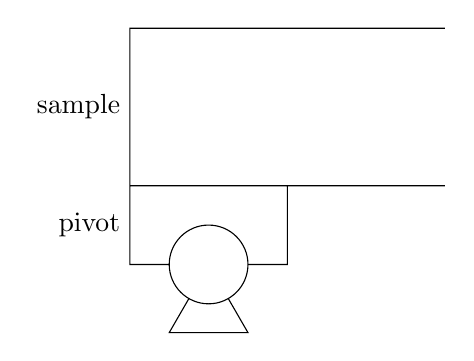
\begin{tikzpicture}
%pivot

\draw
(0,0) circle [radius = 0.5]
(-0.5,0) -- (-1,0) -- (-1,1) -- (1,1) -- (1,0) -- (0.5,0)
(3,1) -- (-1,1) -- (-1,3) -- (3,3);
\draw (-60:0.5) coordinate (start1)
(-120:0.5) coordinate (start2)
(-60:1) coordinate (end1)
(-120:1) coordinate (end2)
(start1) -- (end1) -- (end2) -- (start2);

\draw (-1,2) [left] node {sample}
(-1,0.5) [left] node {pivot};
(-1,-0.5) [left] node {load cell};
\end{tikzpicture}
    }
    \subcaptionbox{After the impact\label{fig:after}}
    {
    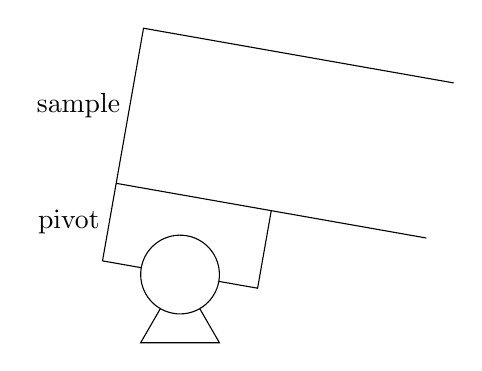
\begin{tikzpicture}[rotate=-10]
%pivot rotated

\draw
(0,0) circle [radius = 0.5]
(-0.5,0) -- (-1,0) -- (-1,1) -- (1,1) -- (1,0) -- (0.5,0)
(3,1) -- (-1,1) -- (-1,3) -- (3,3);

\draw (-50:0.5) coordinate (start1)
(-110:0.5) coordinate (start2)
(-50:1) coordinate (end1)
(-110:1) coordinate (end2)
(start1) -- (end1) -- (end2) -- (start2);

\draw (-1,2) [left] node {sample}
(-1,0.5) [left] node {pivot};
(-1,-0.5) [left] node {load cell};
\end{tikzpicture}
    }
    \caption{Effect of using a pivot instead of a stiff connection}
    \label{fig:pivot}
\end{figure}

\begin{figure}[p]
    \centering
    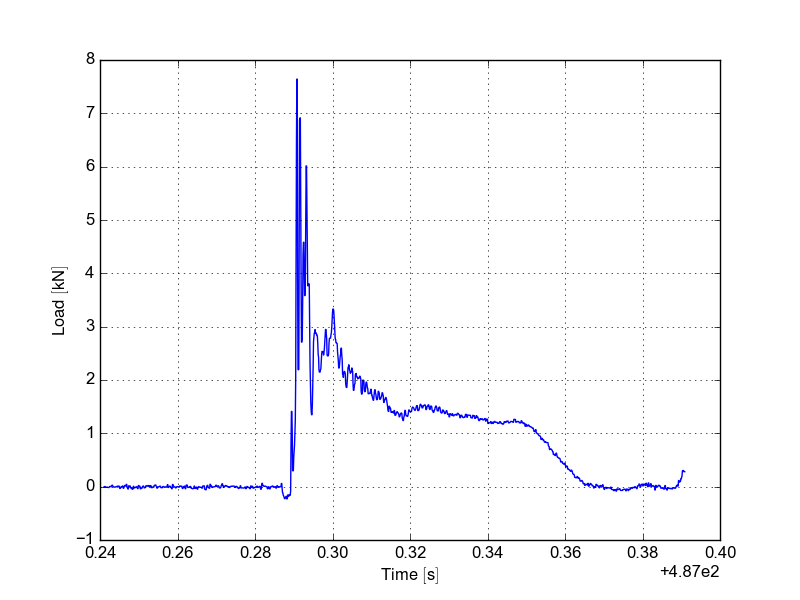
\includegraphics[width = 0.95 \linewidth]{pics/loadip.png}
    \caption{Dip in the force measurement of the load cells at the beginning of the impact}
    \label{fig:dip}
\end{figure}

\begin{figure}
    \centering
    \begin{tikzpicture}
%round sample

%text
\path (90:5) ++ (4,4) coordinate (start)
(-30:5) ++ (4,4) coordinate (end);
\draw [{Latex[length=3mm, width=1mm]}-{Latex[length=3mm, width=1mm]}] (start) arc (90:-30:5)
node [above, sloped,midway] {120\textdegree};


%sample
\draw(4,4) circle [radius=4];

%load cells
\draw (90:3.5) ++ (4,4) circle [radius=.5];
\draw (210:3.5) ++ (4,4) circle [radius=.5];
\draw (-30:3.5) ++ (4,4) circle [radius=.5];

%measurements
\draw[{Latex[length=3mm, width=1mm]}-{Latex[length=3mm, width=1mm]}]
(0,-1) -- (8,-1) node [above,midway] {0,8 m};

%text
\draw (210:5) ++ (4,4) node (load) {load cell}
(4,5) node {impact zone};

%impact zone
\path[clip] (4,4) circle [radius=0.5];
\foreach \x in {2.4,2.6,...,4.6}
\draw[ultra thin] (\x,3.3) -- ++ (2,2);

\end{tikzpicture}
    \caption{Top view of the test setup for the round sample}
    \label{fig:round}
\end{figure}

The specimen have a diameter of 0,8 m. They are placed on pivots on 3 load cells. See \autoref{fig:round}. The pivots enable the specimen to deform more freely as displayed in \autoref{fig:pivot}. In the second campaign the horizontal acceleration of the sample was recorded and found to be significant. Therefore some horizontal movement must occur.

For lighter samples with a thickness below 100 mm a slight dip in the measured load just before impact is recorded. See \autoref{fig:dip}. Probably the sample deforms and reduces the load on the load cells before the impulse is transferred to the load cells. This dip gets less pronounced as the thickness of the samples increases. 
The impact weight is dropped onto the center of the sample. The samples that were tested so far had a thickness of 50, 70 and 100 mm. Only fibre reinforced concrete was used. Unlike suggested by \textcite{c1550} the samples were not sprayed but cast, therefore no accelerators were used in the recipe. The samples were tested by dropping a weight on them once an recording the amount of damage.

\subsection{Square Specimen}
\begin{figure}
    \centering
    \begin{tikzpicture}
%3D square sample


%steel frame
\draw (0,12) rectangle ++(8,-0.3);
\draw (3.8,15.5) -- ++ (6,0)
(3.8,15.2) -- ++ (5.75,0)
(3.8,15.5) -- ++ (0,-0.3)
(3.8,15.2) -- ++ (-2.1,-2.7)
(8,11.7) -- ++ (3.2,4) -- ++ (0,0.3);
\begin{scope}
\pgftransformcm{1}{0}{0.4}{0.5}{\pgfpoint{0}{12cm}}
\draw (0,0) rectangle (8,8);
\draw (1,1) rectangle (7,7);
\end{scope}



%mesh
\begin{scope}
\pgftransformcm{1}{0}{0.4}{0.5}{\pgfpoint{0}{-4.5cm}}
\draw [step=1] (0,0) grid (8,8);
\end{scope}

%concrete slab
\begin{scope}
\pgftransformcm{1}{0}{0.4}{0.5}{\pgfpoint{0}{7cm}}
\draw[fill=lightgray] (0,0) rectangle (8,8);
\draw[fill=black] 
(1.5,1.5) circle [radius = 0.1]
(6.5,1.5) circle [radius = 0.1]
(1.5,6.5) circle [radius = 0.1]
(6.5,6.5) circle [radius = 0.1]; 
\end{scope}
\draw[fill=lightgray] (0,7) rectangle (8,5);
\begin{scope}
\pgftransformcm{0}{1}{0.4}{0.5}{\pgfpoint{8cm}{7cm}}
\draw[fill=lightgray] (0,0) rectangle (-2,8);
\end{scope}
\begin{scope}
\pgftransformcm{1}{0}{0.4}{0.5}{\pgfpoint{4cm}{7cm}}
\draw[fill=white] (0,4) circle [radius = 2];
\end{scope}


%sample
%\draw[fill=gray] 
(0.2,0.25) rectangle ++ (0.5,0.5)
(7.7,0.25) rectangle ++ (0.5,0.5)
(0.5,0) rectangle (7.5,0.5);
\draw[fill=gray]
(0.7,0.25) rectangle (7.7,0.75);

    %side
\begin{scope}
\pgftransformcm{0}{1}{0.4}{0.5}{\pgfpoint{7.5cm}{0cm}}
\draw[fill=gray] (0,0.5) rectangle ++ (0.5,7);
\end{scope}

    %top
\begin{scope}
\pgftransformcm{1}{0}{0.4}{0.5}{\pgfpoint{0}{0.5cm}}
\draw[fill=gray]
(0.5,0.5) -- (7.5,0.5) -- (7.5,7.5) -- (0.5,7.5) --  cycle;
    %bolt
\draw[fill=black] 
(1.5,1.5) circle [radius = 0.1]
(6.5,1.5) circle [radius = 0.1]
(1.5,6.5) circle [radius = 0.1]
(6.5,6.5) circle [radius = 0.1]; 
\end{scope}

%bolts
\draw[ultra thin] 
(2.1,9.5) -- ++ (0,-15) coordinate [pos=0.95] (bolt1)
(7.1,9.5) -- ++ (0,-15) coordinate [pos=0.95] (bolt2)
(4.1,11.5) -- ++ (0,-15) coordinate [pos=0.95] (bolt3)
(9.1,11.5) -- ++ (0,-15) coordinate [pos=0.95] (bolt4);

%Text
\draw
(12,14) node [right,align =left] {steel frame}
(12,7) node [right,align =left] {concrete slab}
(12,2) node [right, align = left] {sample}
(12,-3) node [right,align = left] {mesh}

(5,-6) node (bolts) {bolts};
\draw[-{Latex[length=3mm, width=1mm]}]
(bolts) -- (bolt1);
\draw[-{Latex[length=3mm, width=1mm]}]
(bolts) --(bolt2);
\draw[-{Latex[length=3mm, width=1mm]}]
(bolts) -- (bolt3);
\draw[-{Latex[length=3mm, width=1mm]}]
(bolts) -- (bolt4);

\end{tikzpicture}
    \caption{Sketch of the sample setup for the large scale tests}
    \label{fig:SAMPLE}
\end{figure}


\begin{figure}
    \centering
    
    \subcaptionbox{Top view of concrete slab}{
    \begin{tikzpicture}
%size concrete slab

%concrete slab
\draw (0,0) rectangle (9,9)
(4.5,4.5) circle [radius = 2.1]
(1.5,1.5) circle [radius = 0.1]
(7.5,1.5) circle [radius = 0.1]
(1.5,7.5) circle [radius = 0.1]
(7.5,7.5) circle [radius = 0.1];


\path (225:2.1) -- ++((4.5,4.5) coordinate [at end] (end);

%measurements
\draw [{Latex[length=3mm, width=1mm]}-{Latex[length=3mm, width=1mm]}] 
(0,-1) -- (1.5,-1)
node [midway, above] {0,25 m};
\draw [{Latex[length=3mm, width=1mm]}-{Latex[length=3mm, width=1mm]}] 
(7.5,-1) -- (9,-1)
node [midway, above] {0,25 m};
\draw [{Latex[length=3mm, width=1mm]}-{Latex[length=3mm, width=1mm]}] 
(1.5,-1) -- (7.5,-1)
node [midway, above] {1,0 m};
\draw [{Latex[length=3mm, width=1mm]}-{Latex[length=3mm, width=1mm]}] 
(0,-2) -- (9,-2)
node [midway, above] {1,5 m};

%cut
\draw [dashed]
(0,4.5) -- (4.5,4.5)
node [near start,above] {profile A}
(4.5,1.5) -- (9,1.5)
node [midway,above] {profile B};


\draw [{Latex[length=3mm, width=1mm]}-{Latex[length=3mm, width=1mm]}] 
(10,0) -- (10,1.5)
node [midway, above, sloped] {0,25 m};
\draw [{Latex[length=3mm, width=1mm]}-{Latex[length=3mm, width=1mm]}] 
(10,7.5) -- (10,9)
node [midway, above, sloped] {0,25 m};
\draw [{Latex[length=3mm, width=1mm]}-{Latex[length=3mm, width=1mm]}] 
(10,1.5) -- (10,7.5)
node [midway, above, sloped] {1,0 m};
\draw [{Latex[length=3mm, width=1mm]}-{Latex[length=3mm, width=1mm]}] 
(11,0) -- (11,9)
node [midway, above, sloped] {1,5 m};

%radius
\draw [{Latex[length=3mm, width=1mm]}-]
(end) -- ++ (1.45,1.45);
\path 
(end) -- ++ (2.15, 2.15)  node [pos=1, sloped, above] {R = 0,35 m};



\end{tikzpicture}
    }
    \subcaptionbox{Side view of concrete slab}{
    \begin{tikzpicture}
%side view concrete slab

%text
\draw
(2.25,3.5) node {profile A} 
(6.75,3.5) node {profile B}; 


%measurements
\draw [{Latex[length=3mm, width=1mm]}-{Latex[length=3mm, width=1mm]}] 
(0,-1) -- (2.4,-1)
node [midway, above] {0,4 m};
\draw [{Latex[length=3mm, width=1mm]}-{Latex[length=3mm, width=1mm]}] 
(4.5,-1) -- (2.4,-1)
node [midway, above] {0,35 m};
\draw [{Latex[length=3mm, width=1mm]}-{Latex[length=3mm, width=1mm]}] 
(4.5,-1) -- (7.5,-1)
node [midway, above] {0,5 m};
\draw [{Latex[length=3mm, width=1mm]}-{Latex[length=3mm, width=1mm]}] 
(9,-1) -- (7.5,-1)
node [midway, above] {0,25 m};
\draw [{Latex[length=3mm, width=1mm]}-{Latex[length=3mm, width=1mm]}] 
(0,-2) -- (9,-2)
node [midway, above] {1,5 m};
\draw [{Latex[length=3mm, width=1mm]}-{Latex[length=3mm, width=1mm]}] 
(10,0) -- (10,2.4)
node [midway, above, sloped] {0,4 m};


%left rect
\draw (2.4,0) -- (4.5,0)
(2.4,2.4)-- (4.5,2.4);

%cutLine
\draw[dashed] (4.5, 4) -- ++ (0,-5);

\draw[fill = lightgray] (0,0) rectangle (2.4,2.4)
(4.5,0) -- (9,0) -- (9,2.4) -- (4.5,2.4);

%bolt
\draw [thick] (7.5,0) -- (7.5,2.4)
node [at end, above] {bolt};

\end{tikzpicture}
    }

\caption{Views and dimensions of the concrete slab}
\label{fig:con}
\end{figure}

\begin{figure}
    \centering
    \begin{tikzpicture}
%sample size

%sample
\draw
(0,0) -- (7.8,0) -- (7.8,7.8) -- (0,7.8) -- cycle;

%bolts
\draw 
(0.9,0.9) circle [radius = 0.1]
(0.9,6.9) circle [radius = 0.1]
(6.9,6.9) circle [radius = 0.1]
(6.9,0.9) circle [radius = 0.1];

%measurements
\draw [{Latex[length=3mm, width=1mm]}-{Latex[length=3mm, width=1mm]}]
(0,-1) -- (0.9,-1) node [midway, above] {0,15 m};
\draw [{Latex[length=3mm, width=1mm]}-{Latex[length=3mm, width=1mm]}]
(0.9,-1) -- (6.9,-1) node [midway, above] {1,0 m} ;
\draw [{Latex[length=3mm, width=1mm]}-{Latex[length=3mm, width=1mm]}]
(6.9,-1)--(7.8,-1) node [midway, above] {0,15 m};

\draw [{Latex[length=3mm, width=1mm]}-{Latex[length=3mm, width=1mm]}]
(0,-2) -- (7.8,-2) node [midway, above] {1,3 m} ;


\draw [{Latex[length=3mm, width=1mm]}-{Latex[length=3mm, width=1mm]}]
(8.8,0) -- (8.8,0.9) node [midway, above, sloped] {0,15 m};
\draw [{Latex[length=3mm, width=1mm]}-{Latex[length=3mm, width=1mm]}]
(8.8,0.9) -- (8.8,6.9) node [midway, above, sloped] {1,0 m} ;
\draw [{Latex[length=3mm, width=1mm]}-{Latex[length=3mm, width=1mm]}]
(8.8,6.9)--(8.8,7.8) node [midway, above, sloped] {0,15 m};

\draw [{Latex[length=3mm, width=1mm]}-{Latex[length=3mm, width=1mm]}]
(9.8,0) -- (9.8,7.8) node [midway, above, sloped] {1,3 m} ;
\end{tikzpicture}
    \caption{Top view and dimensions of the specimen}
    \label{fig:spes}
\end{figure}

This test setup was suggested by \textcite{Erik15}. In \autoref{fig:SAMPLE} a 3d sketch of the setup is displayed, please note that it is not to scale and merely serves to illustrate the basic principle. and in \autoref{fig:con} and \autoref{fig:spes} the dimension of the concrete slab and the specimen are given. %Please note that the specimen thickness was one of the variables that was varied in the course of the tests. It ranged between 50 and 100 mm.

The steel frame is only roughly sketched. It serves to attach the mesh to the sample and pretension it. It is bolted into the concrete slab. In \autoref{fig:frame} a picture of the frame already bolted into the sample is given.

\begin{figure}
    \centering
    \includegraphics[width = 0.95\linewidth]{pics/steelframe.jpg}
    \caption{Steel frame mounted on sample}
    \label{fig:frame}
\end{figure}

The concrete slab has several functions. First it simulates the static load resting on the surface support, second as the sample is cast directly on it, the adhesion between rock and shotcrete is simulated. The concrete slab has a round opening in the center with a diameter of 70 cm. This marks the impact zone of the drop weight.  

Both sample and slab are cast from the same concrete, C50, which means it has a uniaxial compressive strength of approximately 50 MPa after 28 days. If fibres are used the fibre content of the concrete is \(40 ~\frac{\text{kg}}{\text{m}^3}\). The sample productions is a two step process. First a concrete slab is cast, which then cures for 28 days, afterwards the sample is cast on top and again cures for 28 days. Afterwards the sample is ready to be tested. 

The adhesive forces between sample and concrete slab are meant to simulate the adhesive forces between shotcrete and rock. Cast concrete is quite smooth but the rock mass surface is quite rough. That is why the surface of the concrete slab has to be roughened before casting the sample. Please also note that the specimen is cast on instead of sprayed on, as it would be \textit{in - situ}. 

The test panel will be attached to the concrete slab with 4 bolts as well. These bolts are simulated by threaded M30 bars, with the previously discussed plates and nuts. The nuts are applied using a torque wrench to keep the applied force consistent. % TO DO description of the bolts and preload force
The intend is to simulate \textit{in - situ} conditions as closely as possible. As well as keep the specimen from simply dropping to the ground after the the adhesive bond breaks. The concrete slab rests on 4 load cells located at the corners. The specimen should only be supported by the bolts and therefore can not have the same outline as the concrete. That is why the edges have to be removed .% and the sample has a cloverleaf shape. If these inward turned corners have any effect on the testing or if they form weak points remains to be seen.
It was also considered to simply remove the corners from the sample, creating a cloverleaf shape. This would have yielded more surface area for the sample. If the resulting inward turned corners have any effect on the testing is not clear.

%The testing method is of yet not defined. For this thesis 2 samples of each type are planned. The current idea would be to start at 1 kJ and increase the load by one kJ with every hit, measure the destruction and see how long the sample survives. This would test both the fatigue resistance and provide a conservative estimate about the maximum survivable impact energy. But this is still being discussed and not decided yet.

\begin{figure}
    \centering
    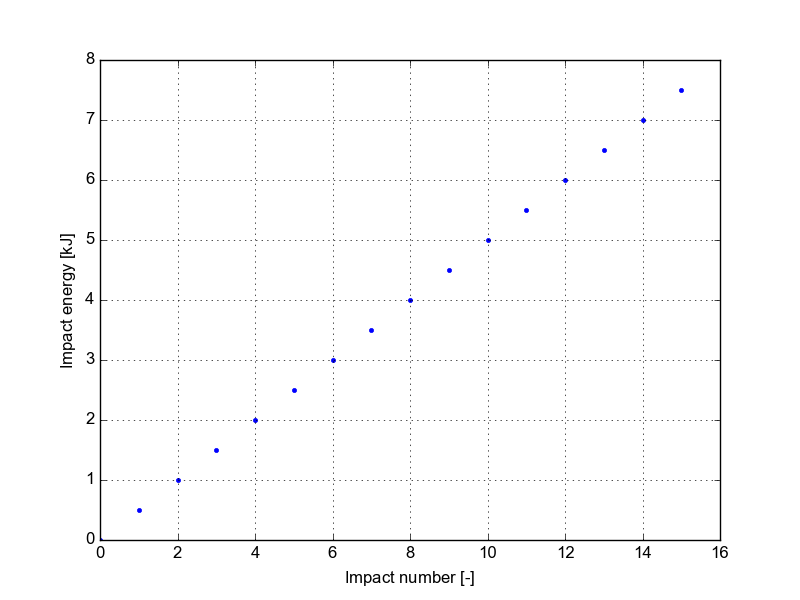
\includegraphics[width = 0.95\linewidth]{pics/impact_energy.png}
    \caption{Energy of each individual impact}
    \label{fig:impactenergy}
\end{figure}

\begin{figure}
    \centering
    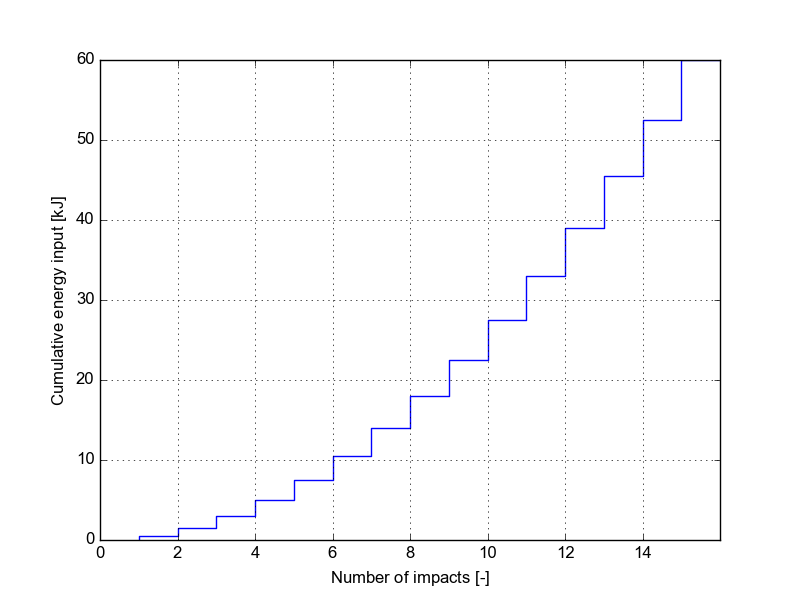
\includegraphics[width = 0.95\linewidth]{pics/cum_energy.png}
    \caption{Total energy}
    \label{fig:cumenergy}
\end{figure}

The testing method is a combination of both categories discussed in \autoref{sec:droptest}. Two samples of a given type are necessary. The first sample will be loaded in multiple impacts. The first impact will have 0,5 kJ and the following impacts will increase by 0,5 kJ.  See \autoref{fig:impactenergy}. The sample probably can with stand an almost endless number of very low energy impacts. Like a concrete wall cannot be destroyed by throwing a tennis ball at it. To keep this from happening the energy of the impacts increases with every hit.
The cumulative energy increases rapidly using this method. See \autoref{fig:cumenergy}.
As the drop weight has a very strong influence on the results of the test, only the 1000 kg drop weight will be used.

This test has two functions. Firstly to show much cumulative energy a sample can survive and secondly to show how the sample handles repeat impacts.

The second sample will be hit by a single impact. This impact will have 50 \% of the cumulative energy the first sample survived. This test will yield information about the largest single impact a sample can survive.

\begin{figure}
    \centering
    \begin{tikzpicture}
%size mesh

%boundary
\path [draw] (0,0) rectangle (4.4,4.6);

%mesh
\draw [help lines, step = .1] (0,0) grid (4.4,4.6);

%bolts
\draw [fill = gray] 
(0.1,0.15) circle [radius= 0.05]
(0.1,2.3) circle [radius= 0.05]
(0.1,4.45) circle [radius= 0.05]

(2.2,.15) circle [radius= 0.05]
(2.2,2.3) circle [radius= 0.05]
(2.2,4.45) circle [radius= 0.05]

(4.3,.15) circle [radius= 0.05]
(4.3,2.3) circle [radius= 0.05]
(4.3,4.45) circle [radius= 0.05];

%measurements
\draw [{Latex[length=3mm, width=1mm]}-{Latex[length=3mm, width=1mm]}] 
(0,-1) -- (4.4,-1)
node [midway, above] {2,2 m};
\draw [{Latex[length=3mm, width=1mm]}-{Latex[length=3mm, width=1mm]}] 
(5.4,0) -- (5.4,4.6)
node[midway, sloped, above] {2,3 m};
\draw[red, dashed, thick]
(-0.2,2.3) -- (2.2,2.3) -- (2.2,-0.2);

\end{tikzpicture}
    \caption{\textit{In-situ} boundary conditions of mesh}
    \label{fig:insituMesh}
\end{figure}

For testing of mesh the boundary conditions are very important. \autocite[5]{villa09} This is especially true for the square sample tests as these try to be as realistic as possible.
The welded mesh currently in use is applied in panels with a size of 2,3 on 2,2 m and a bolt spacing of 1 bolts per meter. See \autoref{fig:insituMesh}. Which means that a 1 x 1 m square of mesh has two open boundaries and two flexible boundaries (illustrated in \autoref{fig:insituMesh} with red dashed lines). Which means that during testing two ends of the mesh should be free and two should be constrained. 
Chain-link and textile mesh can be applied in much larger continuous pieces. Therefore all their boundaries should be confined.

%Therefore this modification to the test rig will allow to vary boundary conditions of the mesh between very stiff and open and even allow pretensioning as needed. The basic principle would be to pull up and attach the mesh to the sides of a concrete slab. %Possible ways of attachment would be addition bolts for example. 
%The drawbacks of this method lie in the very difficult sample preparation, firstly the corners would need to be cut from each sample to give it a clover leaf shape. %as displayed in \autoref{fig:meshBound}. 
%The leaves would need to be bent at a 90 degree angle. This is a lot of preparatory work necessary for a single test. %Ideally the lacing would be attached as one continuous rope and be allowed to glide 

\section{Impact Cushion}

The test weights are made of steel and have sharp edges. During a  seismic impact the accelerated rocks do not strike the surface support directly but first hit a zone of loose and broken rock that forms around the circumference of the excavation which distributes the load across a larger area and cushions the impact slightly. In order to simulate realistic conditions a rubber cushion will be put between drop weight and test panel to distribute the load more evenly. Gravel was also considered as a possible cushion, which would have been even closer to reality and is commonly used in similar tests. The drawback of gravel would be that the energy dissipated through crushing is not known and could vary between experiments, while the deformation energy of a rubber plate should be fairly consistent and calculable.

%As described in the literature review, most cushions used up until now were made from bricks or gravel. For the large scale tests test rubber mats will be used. Rubber mats have to advantage that they have very exactly defined properties. See \autoref{tab:cushion}

\begin{table} [h]
    \centering
    \begin{tabular}{ll}
    \toprule
    Property & typical value \\
    \midrule
    Hardness     &  60  \textdegree IRHD\\
    Density & 1,13 \( \frac{\text{g}}{\text{cm}^3} \) \\
    Tensile strength & 19,5 MPa \\
    Elongation at break & 510 \% \\
    \bottomrule
    \end{tabular}
    \caption{Properties of the rubber cushion after \autocite[76]{metso18}}
    \label{tab:cushion}
\end{table}

The exact material used in this test was Metso Trellex T60. See \autoref{tab:cushion}. Two circles with a diameter of approximately 70 cm and a thickness of 25 mm were glued together to form an impact cushion. 
%TO DO take a nice picture

%As material parameters are already defined and guaranteed by the producer.

\section{Shape of Drop Weight}

As the drop weights have large cutouts on either side for the guide rails, air should be able to escape upward without forming a cushion and slowing the final descend of the weight. These cutouts have the drawback that modelling the drop weight is not a trivial task. A numerical analysis of the drop tests is outside of the scope of this thesis. If a numerical model would be required, the shape of the drop weights would probably have to be changed and channels for air to escape from the impact site would have to be created. Or other steps would have to be taken to make the cross section of the weights more suitable for modelling. 
%TO DO picture or drawing of the drop weight

\section{Sensors}

The main objective of the sensor array is to have at least 100 measurements during the critical part of the experiment. Which means that the first peak of each parameter could be characterized by 100 measurements. Especially load and displacement need to be measured with utmost care. Load displacement curves are the best way to calculate the absorbed energy. \autocite[5]{player04} 
In \autoref{tab:senrequl} the critical times for each parameter and the therefore necessary minimal resolution are given.

\begin{table}[h]
    \centering
    \begin{tabular}{lrr}
    \toprule
         Parameter & Critical time [ms] & Required resolution \\
    \midrule
         Force & 20 & 5 kHz\\
         Displacement & 50 & 2 kHz \\
         Acceleration of drop weight & 20 & 5 kHz \\
         Velocity &  20 & 5 kHz \\
    \bottomrule
    \end{tabular}
    \caption{Required sensor resolutions}
    \label{tab:senrequl}
\end{table}

Therefore the following sensor array was chosen, as displayed in \autoref{tab:senarrl}. According to the suggestion made by \textcite{Erik15} and to have reliable measurements if one of the sensors should malfunction important parameters were measured redundantly. Especially the accelerometer measurements are very versatile. Velocity can be calculated by integrating the measured acceleration over time. Displacement can be calculated by numerically integrating the acceleration over time twice. This was attempted but the results suffered both zero off-set and zero drift. This why they were not included in the analysis. According to \textcite[3]{ansell02} this is both usual and expected.
The force applied by the drop weight can be calculated quite easily: \(F = m * a\). %Of course there is a difference between the force measured by the accelerometer and the load cells, as it is measured in different places.

\begin{table}[h]
    \centering
    \begin{tabular}{lll}
    \toprule
         Parameter & Primary Sensor & Secondary Sensor  \\
    \midrule
         Velocity &  (Accelerometer) & \\
         Force & Load cells & Accelerometer \\
         Displacement & Laser sensor & High speed camera \\
         Acceleration of Drop weight & Accelerometer & \\
         Drop height & Rotary encoder & \\
    \bottomrule
    \end{tabular}
    \caption{Required sensor array}
    \label{tab:senarrl}
\end{table}

\begin{table}
    \centering
    \begin{tabular}{ll}
    \toprule
    Sensor & Type \\
    \midrule
Loadcell & HBM C6A \\
& HBM U10M\\
Laser sensor & SICK 0D1000\\
Accelerometer & Kistler 8704B5000  \\
& PCB 305B03\\
High speed camera & Casio Exilim Pro Ex-F1 \\
& Phantom Miro LC110 \\
Rotary encoder & Leine Linde RHI 503 \\

\bottomrule
    \end{tabular}
    \caption{Overview of the deployed sensors}
    \label{tab:senover}
\end{table}

The sensors chosen for each specific task are listed in \autoref{tab:senover}. %Their technical data sheets are in the Appendix.

The exact sensor array for each test series varies slightly, as it iterated towards the finalized version. The sensor array used in each campaign is described in \autoref{cha:res}. 

As a few sensors were added on later, several Data Logging systems were used which had to be synchronised manually in the post-processing.
The main data logging was done using a HBM MX879B. As main amplifier a HBM MX840B was used. The additional accelerometers were logged using a MREL Data Trap II\textsuperscript{TM}. The signal was amplified using a PCB 480B21. The high speed camera footage was logged by the internal memory of the camera and a standard SD card. 

\subsection{Load Cells}

The load cells are located at the edge of the sample and measure the force of the impact. The difference between the potential energy of the drop weight and this measured is the deformation energy absorbed by the test panel as well as any other kinds of dissipated energy through for example heat or vibrations.

For the round samples, 3 loadcells are used. See \autoref{fig:round}. The sample rests on pivots on top of the load cells. The load cells have a maximum load of 250 kN each. The sampling rate is 10 kHz. 

For the square sample 4 load cells are used. The concrete slab rests on the load cells. The force of the impact by the drop weight travels through the sample and then either directly the through the adhesive contact or the threaded bar bolts into the concrete block and then into the load cells. The load cells have a maximum capacity of 1 MN each.

\subsection{Laser Sensor}
\label{ssec:laser}

The largest displacement was expected at the center of the sample. To not disturb the measurement a non-contact sensor was chosen, a laser distance sensor. 
It is located underneath the sample. As some samples break and pieces could damage the sensor, it has to be protected. That is why it is placed horizontally, slightly away from the center and underneath steel plating and the laser beam reflected by a mirror to hit the center of the sample.

\subsection{Accelerometers}

The test site is underground and humid. Therefore sensors have to be robust. Piezoresistive sensors would give better results, especially when integrating for velocity and displacement, but are more sensitve. Piezoelectric accelerometers can not measure gravity or other constant accelerations, because the piezoelectric sensor element only produces electricity when it experiences a change in acceleration. %Therefore they can only measure changes in acceleration. 
They also have signal decay, which means that the output of the sensor does not immediately drop to zero when the acceleration does. But for the short impacts and high frequencies expected from the drop tests they should be good enough. \autocite{Hanly16} %Especially since they are only secondary sensors.  

Two types of accelerometers were used. 
Both of them are piezoelectric and uniaxial. 
The PCB sensors are more sensitive with \(0,05~\frac{\text{mV}}{(\text{m/s}^2)}\) output and \(\pm 98.000~\frac{\text{m}}{\text{s}^2}\) measuring range.
The Kistler sensors have an output of \(0,1~\frac{\text{mV}}{(\text{m/s}^2)}\) and \(\pm 49.000~\frac{\text{m}}{\text{s}^2}\) measuring range. 
That is why the PCB sensors will be used in positions with higher priority. Except for the drop weight. 
As the thread for a Kistler accelerometer is drilled directly into the weight itself it is impossible to use PCB acceleromters in this position without an adapter.

There are several ways to mount accelerometers. For example using magnets, adhesive or studs. As studs have the best frequency response this mounting method was used primarily. \autocite[24]{Hanly16} The accelerometers on the drop weight were mounted directly. For the other applications steel plates measuring 5 x 5 x 0.8 cm with a hole at the center were manufactured. They were glued in place and the accelerometers were screwed into the central hole.  A slight problem was that the Kistler and PCB accelerometers had different threads, M6 and 1/4" respectively. Using a uniform system would streamline the setup of tests. Exchanging the accelerometers could be considered in future applications.

The drop weight is fitted with an accelerometer that is logged by the main system. In later tests more accelerometers were added. Their respective positions and mounting will be discussed in detail in the description of the set up of each test.

\subsection{Drop Height}

The drop height together with the drop weight is the defining parameter of the kinetic energy available. It is measured by a rotary incremental encoder with a resolution of 500 pulses per revolution. As the testing procedure requires the drop weight to be lowered until it is almost touching the sample. This is done so the measurements of the rotary encoder are reset. The drop height is then calculated from difference between the distance the drop weight is lifted up and the distance it is lowered down. The drop weight is not supposed to touch the sample when it is at the lowest point. This was tested by running a sheet of paper between sample and drop weight.
Due to this constraint imposed by the testing procedure the accuracy of the drop height measurements is significantly lowered compared to the accuracy of the rotary encoder. The accuracy of the drop height measurements is assumed to be $\pm~0,5$ mm. 

\subsection{Drop Weights}

There currently are 5 drop weights available: 50 kg, 100 kg, 200 kg, 500 kg, 1000 kg. The two smallest weights have been modified, their bottom is not flat but optimised to provided a point load.

%TO DO, input a picture of the smaller drop weights
%TO DO, make a sketch of the drop weights

%"Sensor frequency must fit with impact time" Nikolaos Petropoulos in conversation. If you want to measure something that takes almost no time at all, you better have a fucking high measuring frequency! 

\subsection{High Speed Camera}

%TO DO enhance this ugly as fuck graphic!
\begin{figure}
    \centering
    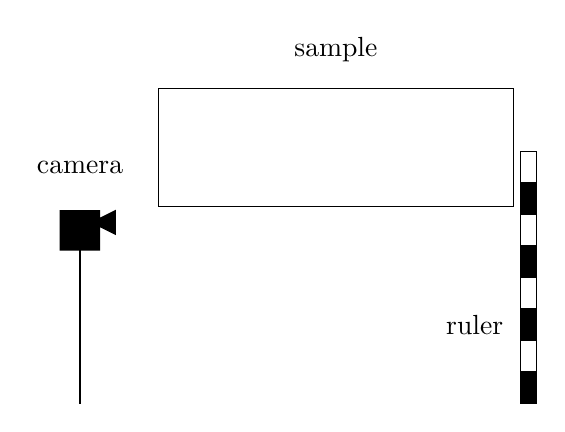
\begin{tikzpicture}
%HORRIBLE camera picture

%displacement
%\draw (1,2.5) parabola bend (3.25,2) (5.5,2.5) node [midway] (down) {this};

%camera
\draw (0,0) -- ++ (0,1.95);
\draw [fill = black]
(-0.25,1.95) rectangle ++ (.5,.5)
(0.25,2.35) -- ++ (0.2,0.1) -- ++ (0,-0.3) -- ++ (-0.2,0.1);

%\draw[ultra thin] (0.25,2.2) -- (5.6,2.4)
%(0.25,2.2) -- (5.6,2);

%sample
\draw
(1,2.5) rectangle ++ (4.5,1.5); 

%ruler
\draw 
(5.6,0) -- (5.6,3.2) -- (5.8,3.2) -- (5.8,0) ;
\foreach \x in {0,0.8, ..., 3.2}
\draw [fill = black]
(5.6,\x) rectangle ++ (0.2,0.4);

%central line
%\draw[ultra thin,dashed] (3.25,4) -- (3.25,0);

%distances
%\draw [{Latex[length=3mm, width=1mm]}-{Latex[length=3mm, width=1mm]}] 
%(0,-1) -- (3.25,-1) node [midway, above] {1,0 m};
%\draw [{Latex[length=3mm, width=1mm]}-{Latex[length=3mm, width=1mm]}] 
%(3.25,-1) -- (5.5,-1) node [midway, above] {0,75 m};
%\draw [{Latex[length=3mm, width=1mm]}-{Latex[length=3mm, width=1mm]}] 
%(0,-2) -- (5.5,-2) node [midway, above] {1,75 m};

%text
\draw (0,3) node {camera}
(3.25,4.5) node {sample}
(5.5,1) node [left] {ruler};

%\draw [{Latex[length=3mm, width=1mm]}-{Latex[length=3mm, width=1mm]}] (3.25,2.5) -- (down);

\end{tikzpicture}
    \caption{Camera set up}
    \label{fig:cam}
\end{figure}

 A Casio Exilim Pro Ex-F1 did all the filming of the tests run for this thesis, it has a maximum frame rate of 1200 frames per second (fps) and a resolution of 336 x 96 Pixel at that setting. At 600 fps the resolution is 432 x 192 Pixel.
As stated in \autoref{tab:senrequl} the minimal resolution for displacement measurement would be 2 kHz. The camera only has 0,8 kHz at its highest setting. Which makes the camera unsuitable as a primary measurement device without compromising the precision goals. But it is useful a secondary sensor, for qualitative assessment and as a confidence check for other sensors.
\begin{comment}
The camera is located approximately one meter away from the center of the sample, where the highest deformations are expected and the rulers are located on the other side of the sample, so about 1,75 m away from the camera. As displayed in \autoref{fig:cam}.


\begin{align*}
\frac{x}{1,0 m} &= \frac{0,01 m}{1,75 m}\\[5pt]
x &= \frac{0,01 m * 1,0 m}{1,75 m} \\
x &= 0,005714 m = 6 mm 
\end{align*}
\label{equ:def}


A quick calculation reveals that the 1 cm deflection measured on the ruler at a distance of 1,75 m is equal to approximately 6 mm of deformation at the center of the sample, 1,0 m away from the camera. As displayed in \autoref{equ:def}
As the expected deformations are quite small this value is assumed to be constant for all deformations. 

%At 1200 fps the 1 cm stripes of the ruler are represented by 3 to 4 pixels. Therefore measurements have an approximate error of \textpm 2 mm from the resolution of the camera alone. At a lower frame rate the error will go down but, but also will the measuring frequency.
\end{comment}

A small literature review revealed that in similar setups much more powerful cameras were used. For example \textcite{Kukolj2018} used a set up with 24,656 fps at 336 x 336 pixels, the application was tracking the propagation of cracks. %A frame rate exceeding 10.000 fps would be sufficient, for the estimated impact time of 20 ms, 200 frames would be available. The camera is located approximately one meter away from the point of expected maximum deformation.

Therefore a stronger high speed camera was sourced. A Phantom Miro LC110. This high speed camera is very sensitive and a safety cage was constructed from polycarbonate sheet and wood to protect it against possible impacts by pieces of a sample.%The resolution at different frame rates is displayed in \autoref{tab:LC110}.
%It was only used in one test and an operator mistake deleted the footage.

\begin{comment}
\begin{table}
    \centering
    \begin{tabular}{ll}
    \toprule
    Resolution & fps \\
    pixel x pixel & \\
    \midrule
    1280 x 720 & 1630 \\
    1280 x 720 & 1810 \\
    896 x 720 & 2520 \\
    640 x 480 & 5090 \\
    512 x 512 & 5790 \\
    384 x 288 & 12.900 \\
    256 x 256 & 19.800 \\
    128 x 128 & 60.400 \\
    128 x 64 & 113.200 \\
    128 x 8 & 400.000 \\
    64 x 8 & 400.000 \\
    \bottomrule
    \end{tabular}
    \caption{Possible resolutions of a Phantom Miro LC110}
    \label{tab:LC110}
\end{table}
\end{comment}

A high speed camera has a high shutter speed, which means that providing sufficient amounts of lights is crucial. Modern powerful lamps use mostly LED because it requires less power to produce the same amount of light when compared to other methods of producing light. 
But it is an inherent property of LED lights that they flicker when connected to an alternating current, for example when connected to the power grid \autocite[74]{steffen07} This flicker has a very high frequency and is not visible to the human eye. But it can distort the footage of high speed camera with a sufficiently high frame rate. Therefore alternative light sources might have to be used if the frame rate is very high. For the experiments conducted for this thesis LED lamps were sufficient. 

The very high amount of light disturbed the laser sensor readings.

Footage with 5000 fps and a resolution of 640 x 480 revealed strong bouncing of the sample which was only hinted at by the previous footage. This bouncing is far from the conditions encountered \textit{in - situ}. \textit{In - situ} the shotcrete is attached to rock and cannot dissipate energy through bouncing.   
%An array of 3 halogen lamps with a total of 26.250 lumen was used.

 


